
%(BEGIN_QUESTION)
% Copyright 2014, Tony R. Kuphaldt, released under the Creative Commons Attribution License (v 1.0)
% This means you may do almost anything with this work of mine, so long as you give me proper credit

A set of three ``87'' relays protects this AC generator against further damage from internal faults.  After years of operating without incident, one day the 52-P and 52-N circuit breakers trip.  Subsequent investigations by electricians reveal a fault in the generator's ``B'' phase winding to ground.  However, the electricians also discover the 41 circuit breaker never tripped as it should have:

$$\includegraphics[width=15.5cm]{i03119x01.eps}$$

Identify the likelihood of each specified fault in this system, to explain why the 41 breaker did not trip when it should have.  Consider each fault one at a time (i.e. no coincidental faults), determining whether or not each fault could independently account for {\it all} observations and symptoms in this circuit.

% No blank lines allowed between lines of an \halign structure!
% I use comments (%) instead, so that TeX doesn't choke.

$$\vbox{\offinterlineskip
\halign{\strut
\vrule \quad\hfil # \ \hfil & 
\vrule \quad\hfil # \ \hfil & 
\vrule \quad\hfil # \ \hfil \vrule \cr
\noalign{\hrule}
%
% First row
{\bf Fault} & {\bf Possible} & {\bf Impossible} \cr
%
\noalign{\hrule}
%
% Another row
125 VDC station power supply dead &  &  \cr
%
\noalign{\hrule}
%
% Another row
CT failed open &  &  \cr
%
\noalign{\hrule}
%
% Another row
41TC coil failed open &  &  \cr
%
\noalign{\hrule}
%
% Another row
86 coil failed open &  &  \cr
%
\noalign{\hrule}
%
% Another row
41a contact failed open &  &  \cr
%
\noalign{\hrule}
} % End of \halign 
}$$ % End of \vbox

\underbar{file i03119}
%(END_QUESTION)





%(BEGIN_ANSWER)

% No blank lines allowed between lines of an \halign structure!
% I use comments (%) instead, so that TeX doesn't choke.

$$\vbox{\offinterlineskip
\halign{\strut
\vrule \quad\hfil # \ \hfil & 
\vrule \quad\hfil # \ \hfil & 
\vrule \quad\hfil # \ \hfil \vrule \cr
\noalign{\hrule}
%
% First row
{\bf Fault} & {\bf Possible} & {\bf Impossible} \cr
%
\noalign{\hrule}
%
% Another row
125 VDC station power supply dead &  & $\surd$ \cr
%
\noalign{\hrule}
%
% Another row
CT failed open &  & $\surd$ \cr
%
\noalign{\hrule}
%
% Another row
41TC coil failed open & $\surd$ &  \cr
%
\noalign{\hrule}
%
% Another row
86 coil failed open &  & $\surd$ \cr
%
\noalign{\hrule}
%
% Another row
41a contact failed open & $\surd$ &  \cr
%
\noalign{\hrule}
} % End of \halign 
}$$ % End of \vbox

%(END_ANSWER)





%(BEGIN_NOTES)

{\bf This question is intended for exams only and not worksheets!}.

%(END_NOTES)


